\documentclass[tikz,border=12pt]{standalone}
\usepackage[T1]{fontenc}
\usepackage{mathpazo}
\usepackage{amsmath,amssymb}
\usepackage{xcolor}
\usetikzlibrary{arrows.meta,calc}

%% ── Colour palette ───────────────────────────────────────────────────────
\definecolor{panelgreen} {RGB}{238,248,238}   % near-white, soft green tint
\definecolor{panelblue}  {RGB}{234,242,254}   % near-white, soft blue tint
\definecolor{accentgreen}{RGB}{  0,130,100}   % thin top-rule accent (left)
\definecolor{accentblue} {RGB}{ 40, 60,175}   % thin top-rule accent (right)
\definecolor{tealpoint}  {RGB}{  0,128,112}
\definecolor{bluepoint}  {RGB}{ 38, 55,160}
\definecolor{diagcol}    {RGB}{175,175,175}
\definecolor{arrowcol}   {RGB}{ 50, 50, 50}
\definecolor{labelgray}  {RGB}{ 90, 90, 90}

%% ── TikZ styles ──────────────────────────────────────────────────────────
\tikzset{
  %% Clean card: very light fill, hairline border, small rounded corners
  panel/.style={
    draw=black!14, line width=0.5pt,
    rounded corners=6pt
  },
  %% Thin coloured top rule (drawn separately for each panel)
  accrule/.style={line width=2.2pt, line cap=round},
  frame/.style={draw=black!20, line width=0.6pt},
  axis/.style={
    draw=black!60, line width=1.0pt,
    -{Latex[length=3.6pt,width=2.6pt]}
  },
  diag/.style={
    draw=diagcol, dashed,
    dash pattern=on 4.5pt off 3pt,
    line width=0.72pt
  },
  leftpoint/.style={
    circle, fill=tealpoint, draw=white,
    line width=0.7pt, inner sep=0pt, minimum size=9.5pt
  },
  rightpoint/.style={
    circle, fill=bluepoint, draw=white,
    line width=0.55pt, inner sep=0pt, minimum size=7.5pt
  },
  axislabel/.style={font=\large\itshape, text=labelgray},
  paneltitle/.style={font=\Large},
}

\begin{document}
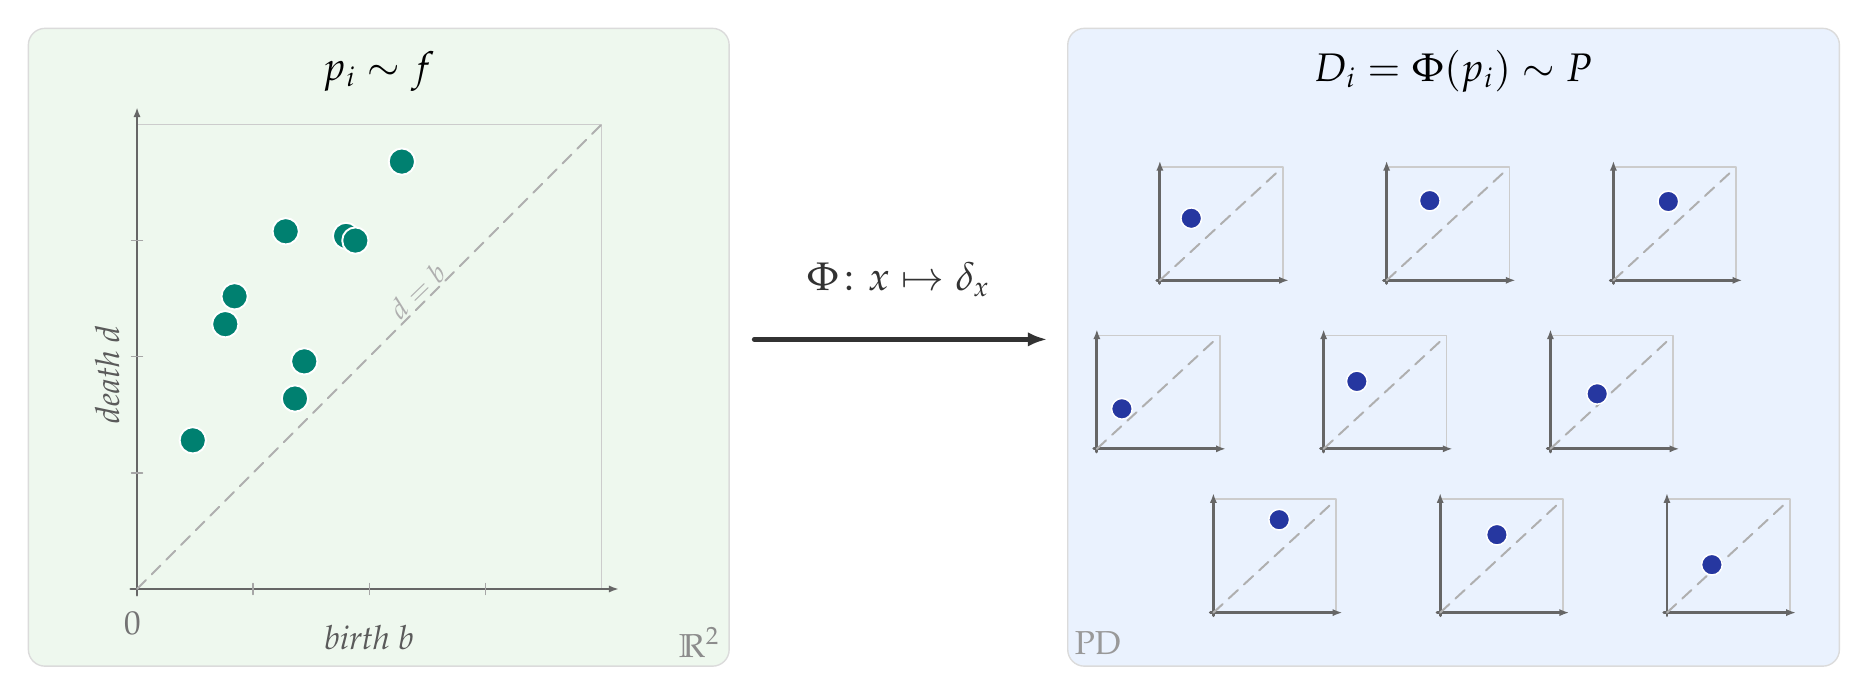
\begin{tikzpicture}[x=1cm, y=1cm, line cap=round, line join=round]

  %% ── Layout constants ──────────────────────────────────────────────────
  \def\LW{8.90}    % left panel width
  \def\LH{8.10}    % left panel height
  \def\RX{13.20}   % right panel x-origin
  \def\RW{9.80}    % right panel width
  \def\RH{8.10}    % right panel height
  \def\PS{5.90}    % scatter-plot inner size
  \def\AY{4.15}    % arrow vertical centre

  %% ══════════════════════════════════════════════════════════════════════
  %%  LEFT PANEL
  %% ══════════════════════════════════════════════════════════════════════
  \path[fill=panelgreen, panel] (0,0) rectangle (\LW,\LH);


  %% Panel title
  \node[paneltitle] at (\LW/2, \LH-0.55) {$p_i \sim f$};

  %% ── Scatter plot ──────────────────────────────────────────────────────
  \begin{scope}[shift={(1.38,0.98)}]
    \draw[frame] (0,0) rectangle (\PS,\PS);
    \draw[axis]  (-0.08,0)  -- (\PS+0.22,0);
    \draw[axis]  (0,-0.08)  -- (0,\PS+0.22);
    \draw[diag]  (0,0)      -- (\PS,\PS);

    %% Axis labels
    \node[axislabel, anchor=north] at (\PS/2, -0.34) {birth $b$};
    \node[axislabel, anchor=east, rotate=90]
          at (-0.38, \PS/1.7) {death $d$};

    %% Diagonal label
    \node[axislabel, rotate=44, anchor=south west, font=\normalsize\itshape,
          text=diagcol]
          at (0.57*\PS-0.02, 0.57*\PS-0.14) {$d = b$};

    %% Tick marks
    \foreach \t in {0.25, 0.50, 0.75}{
      \draw[black!35, line width=0.5pt]
            ({\t*\PS},-0.07) -- ({\t*\PS}, 0.07);
      \draw[black!35, line width=0.5pt]
            (-0.07,{\t*\PS}) -- ( 0.07,{\t*\PS});
    }

    %% Sample points
    \foreach \xn/\yn in {
      0.12/0.32, 0.19/0.57, 0.21/0.63, 0.32/0.77,
      0.36/0.49, 0.45/0.76, 0.47/0.75, 0.34/0.41, 0.57/0.92
    }{
      \node[leftpoint] at ({\xn*\PS},{\yn*\PS}) {};
    }
  \end{scope}

  %% Corner labels
  \node[font=\large\bfseries, text=black!55] at (1.32,0.54) {$0$};
  \node[font=\large,           text=black!45] at (\LW-0.38,0.30)
        {$\mathbb{R}^2$};

  %% ══════════════════════════════════════════════════════════════════════
  %%  MIDDLE ARROW
  %% ══════════════════════════════════════════════════════════════════════
  \draw[-{Latex[length=7pt,width=5.2pt]},
        line width=1.8pt, color=arrowcol]
        (\LW+0.32, \AY) -- (\RX-0.26, \AY);

  \node[font=\Large, text=arrowcol]
        at ({(\LW+\RX)/2}, \AY+0.76)
        {$\Phi\colon x \mapsto \delta_x$};

  %% ══════════════════════════════════════════════════════════════════════
  %%  RIGHT PANEL
  %% ══════════════════════════════════════════════════════════════════════
  \path[fill=panelblue, panel]
        (\RX,0) rectangle ({\RX+\RW},\RH);


  \node[paneltitle] at ({\RX+\RW/2}, {\RH-0.55})
        {$D_i = \Phi(p_i) \sim P$};

  %% ── Micro-plot macro ─────────────────────────────────────────────────
  \newcommand{\microplot}[4]{%
    \begin{scope}[shift={({\RX+#1},{#2})}]
      \draw[frame] (0,0) rectangle (1.56,1.44);
      \draw[axis]  (-0.04,0)   -- (1.64,0);
      \draw[axis]  (0,-0.04)   -- (0,1.52);
      \draw[diag]  (0,0)       -- (1.54,1.42);
      \node[rightpoint]
            at ({0.18 + 1.15*(#3)},{0.15 + 1.12*(#4)}) {};
    \end{scope}%
  }

  %% 3 × 3 grid
  % row 3 (top)
  \microplot{1.17}{4.90}{0.19}{0.57}
  \microplot{4.05}{4.90}{0.32}{0.77}
  \microplot{6.93}{4.90}{0.45}{0.76}
  % row 2 (middle)
  \microplot{0.37}{2.76}{0.12}{0.32}
  \microplot{3.25}{2.76}{0.21}{0.63}
  \microplot{6.13}{2.76}{0.36}{0.49}
  % row 1 (bottom)
  \microplot{1.85}{0.68}{0.57}{0.92}
  \microplot{4.73}{0.68}{0.47}{0.75}
  \microplot{7.61}{0.68}{0.34}{0.41}

  %% Corner label
  \node[font=\large, text=black!40] at (\RX+0.38,0.30) {PD};

\end{tikzpicture}
\end{document}
